	Das dynamische Verhalten des Systems wird mittels Sequenzdiagrammen modelliert.
	Hier wird zunächst ein grobes, geräteübergreifendes Diagramm vorgestellt.
	Die restlichen Sequenzdiagramme beziehen sich nur auf wichtige Methoden in den gekapselten Ökosystemen APP, Website und Backend. Im Weiteren werden Lost und Found Messages verwendet, um die Kommunikation der App und Website mit dem Server zu visualisieren. 
	
\section*{Geräteübergreifendes Sequenzdiagramm}

\begin{figure}[h]
	\centering
	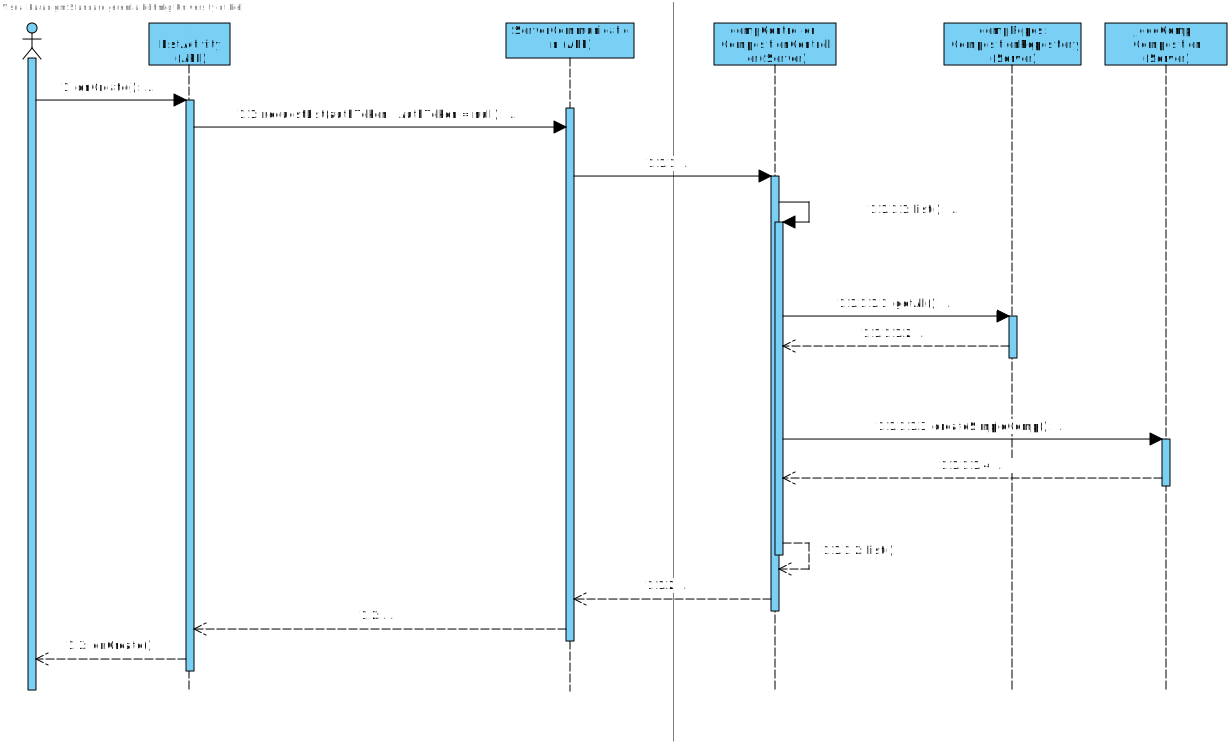
\includegraphics[width=\textwidth]{img/Diagramme/Sequenz/Overview}
	\caption{Sequenzdiagramm}
	\label{fig:sequenz-overview}
\end{figure}
\noindent
Zusammengefasst beschreibt dieses Diagramm das grobe Verhalten des Systems, das abläuft, wenn ein Nutzer über die App sich die für ihn anzeigbaren Kompositionen auflisten lässt. Dabei bezieht es die Kommunikation zwischen Android App und Backend mit ein.\newline

\noindent Der Benutzer öffnet die App, wodurch die Methode onCreate() der ListActivity aufgerufen wird. Beim Start sendet die App ein HTTPS-Request an den Server. Daraufhin fragt der Server die Daten aus der Datenbank ab und erstellt aus diesen ein versendbares Objekt in Form einer Liste von SimpleComp-Objekten. Diese schickt das Backend im Rahmen der Antwort auf den GET-Request an die App, welche die erhaltenen Daten verarbeitet, worauf sie diese dem Benutzer anzeigen kann.

\section*{Sequenzdiagramme der App}
\subsection*{ Öffnen der ListActivity}

\begin{figure}[h]
	\centering
	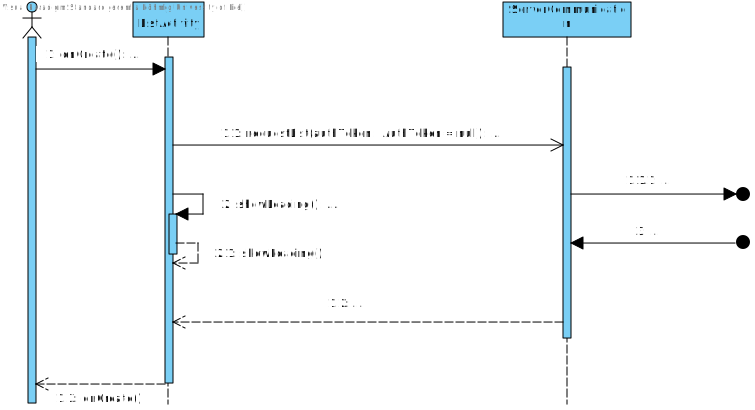
\includegraphics[width=\textwidth]{img/Diagramme/Sequenz/App_list}
	\caption{Sequenzdiagramm - Öffnen der ListActivity}
	\label{fig:sequenz-app_list}
\end{figure}
\noindent
Dieses Sequenzdiagramm zeigt den Vorgang, der abläuft, wenn die ListActivity initial gestartet wird und mit einer Liste aus Kompositionseinträgen zu füllen ist.\newline

\noindent Der Ablauf der Aktivitäten beginnt mit dem Start der ListActivity, bei dem ein Rufen der Standard-Methode onCreate() erfolgt. Da der Nutzer noch nicht eingeloggt ist, startet die App eine requestList()-Anfrage ohne Token. Diese läuft in einem eigenen Thread, damit der UI-Thread nicht blockiert. Die Methode requestList() führt einen HTTPS-Request an das Backend aus. In der Zeit, in der die ListActivity die Antwort noch nicht erhalten hat, zeigt sie mithilfe von showLoading() eine Ladeanimation an.
\pagebreak
\subsection*{ Klicken auf Kompositionseintrag}

\begin{figure}[h]
	\centering
	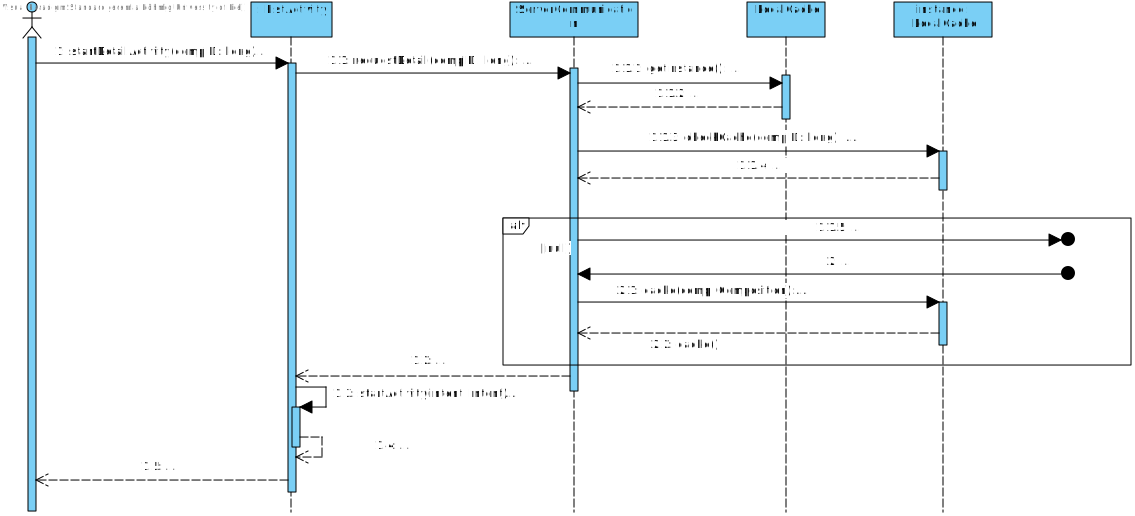
\includegraphics[width=\textwidth]{img/Diagramme/Sequenz/App_detail}
	\caption{Sequenzdiagramm - Klick auf Kompositionseintrag}
	\label{fig:sequenz-App_detail}
\end{figure}


\noindent Fortführend schließt sich dieses Sequenzdiagramm an den Usage-Flow des obigen an. Ist die Liste geladen, will der Nutzer sich früher oder später eine der Kompositionen  detailliert als Grafik anzeigen lassen. Hierfür reicht ein Tippen auf das jeweilige Listenelement aus, um die Detailansicht in Form der DetailActivity aufzurufen.\newline
\\
Durch die genannte UI-Aktion wird die Methode startDetailActivity() aufgerufen, was die statische Methode requestDetail() veranlasst, im LokalCache nach der gewünschten Komposition zu suchen.
Falls diese noch nicht im Cache ist, sendet die App eine HTTPS-Request an den Server.
In der Antwort auf diesen Request sind alle nötigen Details der Komposition enthalten, wozu unter anderem ihre Nodes zählen.
Die Details werden in der Komposition gespeichert, die wiederum im LokalCache abgelegt ist, und so auch an die ListActivity zurückgegeben. Diese übergibt die nun mit Details ausgestattete Komposition an einen Intent, der zum Starten der DetailsActivity dient.\newline
\\
Da LocalCache ein Singleton ist, muss man zu Beginn die Instanz abrufen. Wir planen, die Instanz vorzudefinieren (eager instantiation), wodurch der Fall, dass man die Instanz erst erzeugen müsste, nie eintritt.\newline
\\ \noindent
Die Methode httpsRequest() wird nicht implementiert, sondern dient hier zur Abstraktion. In der Implementation wird diese Abfrage asynchron erfolgen und in einem anderen Thread laufen, so dass sie den UI-Thread nicht blockiert. 


\pagebreak
\section*{Sequenzdiagramme des Servers}


\begin{figure}[h]
	\centering
	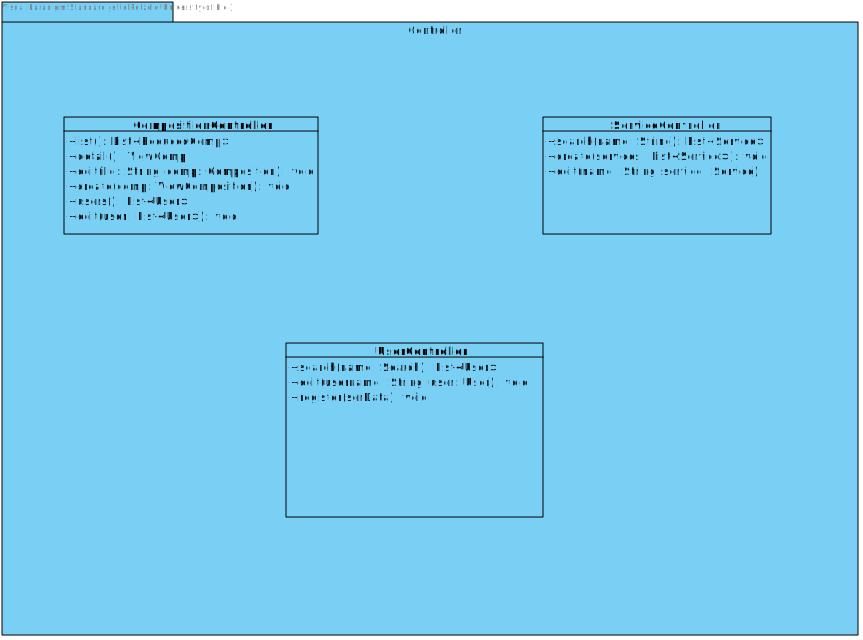
\includegraphics[width=\textwidth]{img/Diagramme/Sequenz/Controller}	
	\caption{Sequenzdiagramm - Kompositionsanfrage}
	\label{fig:sequenz-a}
\end{figure}
\noindent
Nach der Betrachtung der Android-App folgt nun eine detailliertere Darstellung, wie sich die Server-Seite verhält, wenn eine Komposition in Detailansicht angefragt wird.\\ \\ 
\noindent Eine solche Anfrage wird vom CompositionsController entgegengenommen.
Die angefragte Komposition wird in der Datenbank nachgeschlagen (über das CompositionRepository) und als Composition-Objekt zurückgegeben.
Anschließend wird eine DetailComp erstellt, welche die benötigten Daten für das Frontend enthält. 
Um diese zu erstellen, müssen zunächst alle CompositionNodes und danach alle CompositionEdges in versendbare Objekte (Nodes und Edges) umgewandelt werden. 
Dabei wird für jede Kante noch die Kompatibilität überprüft und mögliche Alternativen werden gesucht und ggf. gespeichert. Zurückgeliefert wird also eine DetailComp, die in allen Kanten eine CompatibilityAnswer enthält.\newline
\\ \noindent
Wir haben uns dafür entschieden, eine Util-Klasse zur Berechnung der Compatibility zwischen zwei verschiedenen Diensten (repräsentiert durch ihre IDs) zu verwenden.
Da auch HTTPS-Requests erwartet werden, die nur zu zwei einzelnen Diensten die Kompatibilität erfahren wollen, wäre eine Implementierung dieser Funktion in der Edge-Klasse nicht praktikabel.\newline
\\ \noindent
Da es sich bei dem durch dieses Sequenzdiagramm modellierten dynamischen Verhalten um das komplexeste unseres Backends handelt und sich viele andere Abläufe in ihm widerspiegeln, sei nur dieses als Repräsentant der Arbeitsweise aufgeführt.

\newpage
\section*{Sequenzdiagramme des Web Frontends}
\subsection*{ Erstellen einer Komposition}

\begin{figure}[!h]
	\centering
	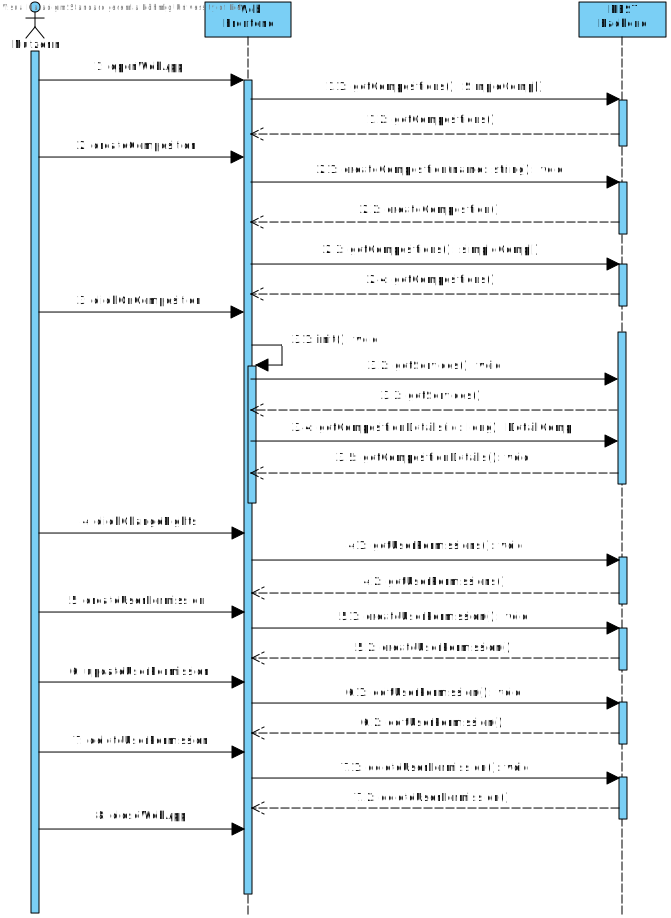
\includegraphics[width=.5\textwidth]{img/Diagramme/Sequenz/Frontend_createComp}
			
	\caption{Sequenzdiagramm - Erstellen einer Komposition}
	\label{fig:sequenz-createComp}
\end{figure}

\noindent
Um eine neue Komposition zu erstellen, fragt das Web Frontend zunächst die dem Nutzer verfügbaren Kompositionen vom Backend an und stellt diese bei Erhalt der Antwort dar. Über ein Eingabefeld lässt sich ein Name für eine neue Komposition festlegen und mit einem zusätzlichen Knopf erstellen. Hiernach wird die Liste der verfügbaren Kompositionen aktualisiert. Ein Klick auf die Komposition löst das Abrufen der bisher nicht erhaltenden Kompositionsdetails vom Backend aus. Erhält das Frontend diese, zeigt es sie in der Bearbeitungsansicht an. Als Autor der Komposition lassen sich nun die Listen mit den Nutzenden einsehen und bearbeiten, die diese Komposition betrachten oder bearbeiten dürfen. Hierbei fordert das Web Frontend alle Informationen immer aus dem Backend an, beziehungsweise schickt Aktualisierungen vom Nutzenden an das Backend.

\newpage
\subsection*{ Bearbeiten einer Komposition}

\begin{figure}[!h]
	\centering
	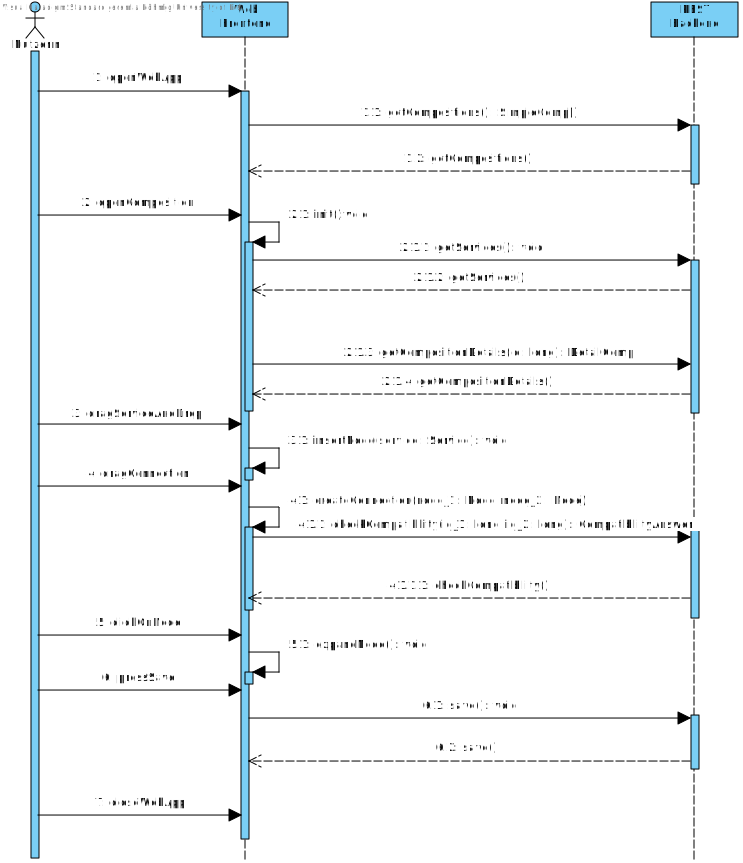
\includegraphics[width=.5\textwidth]{img/Diagramme/Sequenz/Frontend_editComp}			
	\caption{Sequenzdiagramm - Bearbeiten einer Komposition}
	\label{fig:sequenz-editComp}
\end{figure}
\noindent
Um eine Komposition zu bearbeiten, fragt das Frontend zunächst wieder die dem Nutzer verfügbaren Kompositionen vom Backend an und stellt diese dar. Ein Klick auf die Komposition lässt die Details sowie Services vom Backend abrufen und in der Bearbeitungsansicht anzeigen. Indem man einen Service aus dem SidePanel in das Canvas zieht, erstellt man lokal einen Knoten. Das Verbinden von zwei Knoten erstellt zunächst lokal eine Verbindung, wobei eine Anfrage an das Backend geht, die das Überprüfen der Kompatibilität überprüfen lässt. Beim Klicken auf einen Knoten wird eine Detailansicht für den verwendeten Dienst angezeigt. Wiederum sendet ein Klick auf Speichern die aktualisierte Komposition an den Server.

\newpage
\subsection*{ Bedienung des Adminpanels}

\begin{figure}[!h]
	\centering
	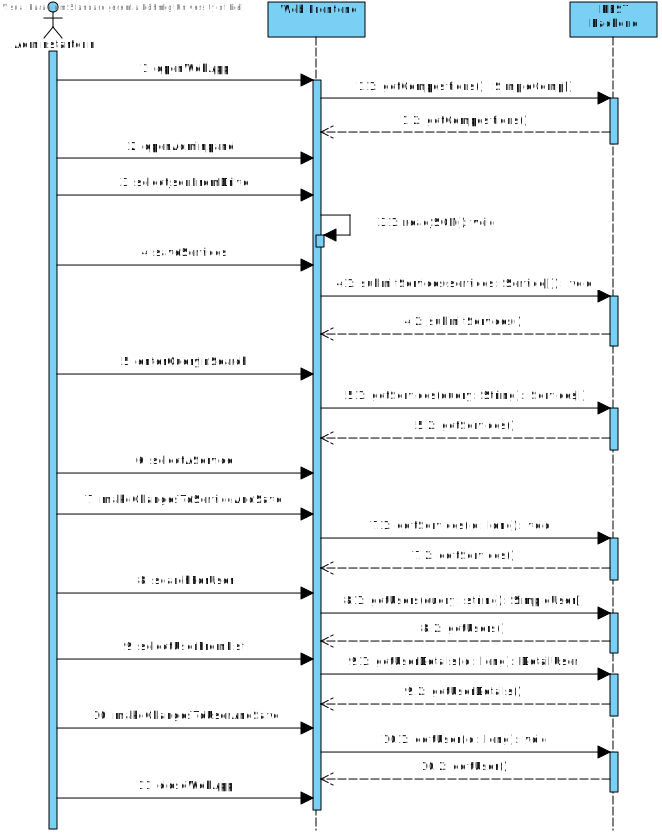
\includegraphics[width=.5\textwidth]{img/Diagramme/Sequenz/Frontend_admin}			
	\caption{Sequenzdiagramm - Bedienung des Adminpanels}
	\label{fig:sequenz-adminPanel}
\end{figure}
\noindent
Das Adminpanel lässt sich aus der Kompositionsübersicht erreichen. Über eine Maske lässt sich eine JSON-Datei mit Services einlesen, die zunächst nur lokal zwischengespeichert und dann bei Bestätigung an das Backend übermittelt werden. Ein Suchfeld für Dienste erlaubt, eine Suchanfrage an das Backend zu schicken und durch Auswählen eines Listeneintrags die Details eines Services zu bearbeiten, die das Frontend bei Bestätigung der Eingabe an das Backend übermittelt. Weiterhin ermöglicht das Frontend die Suche nach registrierten Nutzenden. Wiederum fragt das Auswählen eines Nutzers die Details vom Backend ab, die ein Administrierender bearbeiten kann. Nach Bestätigung der Änderungen sendet das Frontend die angepassten Daten an das Backend, welches sie speichert.
